\section{Arquitectura clásica de RPC}

Una llamada a procedimiento remoto (RPC) es un protocolo de comunicación entre procesos que permite a un programa solicitar la ejecución de un procedimiento que reside en otro espacio de direcciones, ocultando al programador los detalles del transporte de red~\cite{birrell1984rpc}. La arquitectura clásica de RPC se compone de cinco elementos: el \textbf{cliente}, que invoca el procedimiento como si fuera local; el \textbf{stub del cliente}, que empaqueta (\emph{marshalls}) los parámetros; el \textbf{tiempo de ejecución de RPC} (\emph{runtime}), que gestiona el transporte por red; el \textbf{stub del servidor}, que desempaqueta los parámetros y llama al procedimiento real; y el \textbf{servidor}, que ejecuta la lógica y devuelve el resultado~\cite{coulouris2011distributed,tanenbaum2007distributed}. Las tres prácticas de este reporte comparten esta misma rejilla conceptual y difieren únicamente en cómo cada tecnología concreta realiza cada uno de los cinco componentes.

\section{Semánticas de invocación}

La falibilidad de la red obliga a definir explícitamente qué ocurre cuando una petición o su respuesta se pierden. Se reconocen tres semánticas de invocación:

\begin{itemize}
    \item \textbf{At-least-once (al menos una vez):} el cliente reintenta hasta recibir confirmación; si el servidor ya procesó la primera petición, el procedimiento podría ejecutarse más de una vez. Solo es segura si la operación es idempotente.
    \item \textbf{At-most-once (a lo sumo una vez):} el sistema filtra duplicados mediante identificadores de transacción y, ante un fallo, prefiere reportar el error a ejecutar la operación dos veces.
    \item \textbf{Exactly-once (exactamente una vez):} combina los reintentos del esquema \emph{at-least-once} con el filtrado de duplicados del esquema \emph{at-most-once}; en el caso general es imposible de garantizar, pero puede aproximarse con almacenamiento durable y claves de idempotencia.
\end{itemize}

\section{Alcance del documento y entorno de ejecución común}

Las tres prácticas se desarrollan sobre un contenedor Docker con imagen \texttt{fedora:36}, en vez de sobre una instalación nativa del sistema operativo anfitrión. Esta decisión responde a una razón técnica concreta: el instructivo especifica comandos de administración basados en \texttt{dnf}/systemd propios de Fedora (gestor de paquetes, unidades de \texttt{systemd} para \texttt{nginx} y \texttt{fcgiwrap}), mientras que el equipo de trabajo utilizado ejecuta una distribución basada en Arch Linux con un gestor de paquetes distinto (\texttt{pacman}). Encapsular el entorno en un contenedor con la distribución exacta que pide el instructivo garantiza reproducibilidad total de los comandos documentados, aísla las dependencias de la práctica del resto del sistema anfitrión, y permite compartir la misma imagen base entre las tres prácticas sin necesidad de una máquina virtual completa. La Tabla~\ref{tab:entorno-comun} resume las características de este entorno.

\begin{table}[H]
\centering
\caption{Entorno de ejecución común a las tres prácticas.}
\label{tab:entorno-comun}
\begin{tabularx}{\linewidth}{lX}
\toprule
\textbf{Componente} & \textbf{Detalle} \\
\midrule
Anfitrión & CachyOS Linux (derivada de Arch, \emph{rolling release}) con Docker 29.6.2 \\
Motor de contenedores & Docker \\
Imagen base & \texttt{fedora:36} \\
Aislamiento de red & Publicación de puertos por contenedor (\emph{port mapping}) hacia \texttt{localhost} del anfitrión \\
\bottomrule
\end{tabularx}
\end{table}

\begin{figure}[H]
\centering
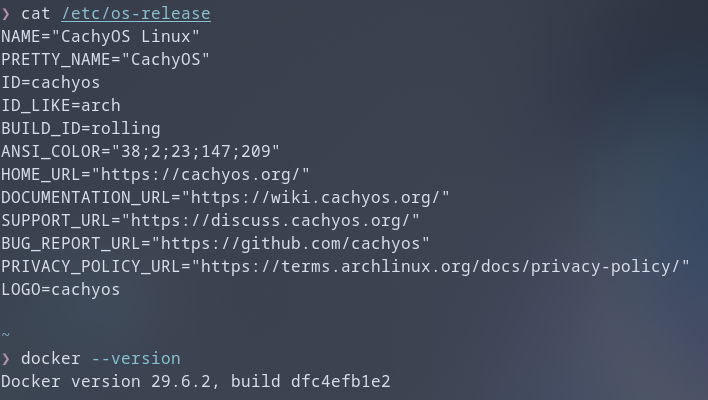
\includegraphics[width=0.8\linewidth]{../src/ss/1.1.png}
\caption{Identificación del sistema operativo anfitrión (\texttt{/etc/os-release}) y versión de Docker.}
\label{fig:host-info}
\end{figure}

La Figura~\ref{fig:host-info} documenta la incompatibilidad que motiva el uso de contenedores: el campo \texttt{ID\_LIKE=arch} confirma que el anfitrión pertenece a la familia Arch Linux, cuyo gestor de paquetes (\texttt{pacman}) y esquema de versiones continuas (\texttt{BUILD\_ID=rolling}) difieren de los que asume el instructivo (Fedora, \texttt{dnf}, versiones puntuales). Docker resuelve esta brecha ejecutando el espacio de usuario completo de Fedora~36 sobre el kernel del anfitrión, sin la sobrecarga de virtualizar hardware como haría una máquina virtual.
